\chapter{Fundamentação teórica}\label{cap:fundamentacao_teorica}

Este capítulo apresenta a base conceitual necessária para o entendimento e o desenvolvimento deste trabalho, estabelecendo as diretrizes técnicas que fundamentam o projeto do processador proposto. Para tanto, abordam-se inicialmente os aspectos históricos da computação e a evolução das estruturas de processamento, seguidos pelas principais filosofias de Arquiteturas de Conjuntos de Instruções (ISA, do inglês \textit{Instruction Set Architecture}), especialmente as especificações do conjunto básico RV32I da arquitetura RISC-V e os componentes que integram o modelo de ciclo único. Por fim, apresenta-se uma revisão de trabalhos correlatos, identificando soluções existentes na literatura que serviram de referência.

Desde as primeiras civilizações humanas, existe a necessidade de quantificar e calcular. Ao longo da história, diversos objetos e métodos foram utilizados para esse fim, passando por pedras, ossos, contas, símbolos, engrenagens e, eventualmente, a energia elétrica \cite{silva2024arquitetura}. Com o avanço da sociedade, a demanda por cálculos mais complexos e em larga escala impulsionou o desenvolvimento de novas ferramentas, fazendo surgir a máquina de calcular chamada computador. Atualmente, o termo "computador"\ é utilizado para designar todos os dispositivos eletrônicos programáveis que realizam operações matemáticas e lógicas \cite{harper_computer}.

Em meados de 1934, Charles Babbage projetou a máquina analítica, considerada o primeiro computador mecânico de uso geral. Esse projeto estabeleceu um fundamento essencial para os computadores atuais, cujo ciclo de funcionamento consiste em ler dados, armazenar, calcular e gerar saídas. Apesar de simples, essa lógica de operação serve como base para a computação moderna \cite{silva2024arquitetura}, sendo conceitos fundamentais até os dias de hoje, inclusive no desenvolvimento deste trabalho.

Outro grande marco importante para a evolução da área foi o lançamento do Harvard Mark I em 1944, desenvolvido por uma equipe de engenheiros da IBM liderada pelo professor da Universidade de Harvard Howard H. Aiken. O Mark I definiu um dos conceitos mais fundamentais da computação: a divisão da estrutura interna do processador, componente responsável por executar todos os cálculos e operações do computador, em cinco partes: Unidade de Controle (CU, do inglês \textit{Control Unit}), Unidade Lógica e Aritmética (ALU, do inglês \textit{Arithmetic Logic Unit}), Memória de Dados, Memória de Instruções e Entrada/Saída (I/O, do inglês \textit{Imput/Outup}). Essa divisão ficou conhecida como arquitetura de Harvard, cujo modelo é ilustrado na Figura \ref{fig:arquitetura_harvard} \cite{silva2024arquitetura}. Para este trabalho, esse modelo será adotado por facilitar a implementação de um processador de ciclo único.

\begin{figure}[!htb]%% Ambiente figure
     \centering %% Centraliza a imagem no documento (recomendado)
     \caption{Arquitetura Harvard}%% Legenda da sua figura
     \label{fig:arquitetura_harvard}%% Rótulo para você citar no texto com \ref{fig:arquitetura_harvard}
     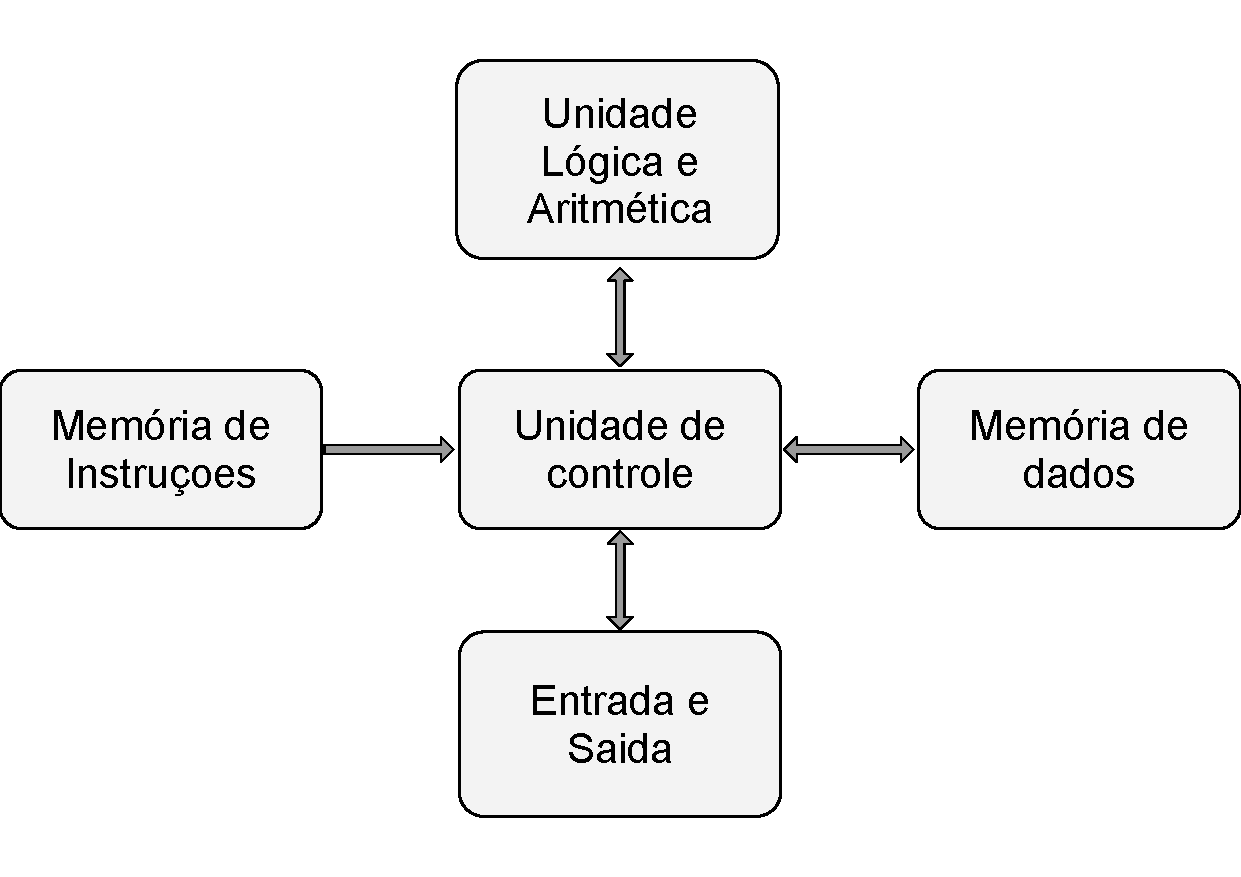
\includegraphics[scale=0.5]{figuras/arquiteturaHarvard.pdf}
     \fonte{Adaptado de \citeonline{silva2024arquitetura}}%% Fonte adaptada
\end{figure}

A CU, apresentada na Figura \ref{fig:arquitetura_harvard}, é responsável por gerenciar toda a comunicação interna do processador, coordenando o fluxo de dados entre os demais componentes. Para cada operação, a CU busca a informação na memória de instruções, decodifica-a e comanda sua execução. Esse processo pode ser projetado de diferentes maneiras: executando toda a instrução em um único período, como no modelo de ciclo único; dividindo a operação em várias etapas, como no modelo multiciclo; ou processando múltiplos estágios de instruções distintas simultaneamente, como na técnica de pipeline \cite{silva2024arquitetura}.

Dentre essas abordagens, a arquiteturas pipeline e suas variações são as mais utilizadas em processadores comerciais modernos, devido ao maior desempenho proporcionado pela execução sobreposta de instruções. O modelo multiciclo, embora tenha sido amplamente empregado em gerações anteriores de processadores, atualmente possui uso mais restrito. Já o modelo ciclo único apresenta o menor desempenho entre os três e não é utilizada comercialmente apenas no âmbito acadêmico \cite{ciclo_instrucao}.

Apesar de suas limitações de desempenho, a arquitetura ciclo único é amplamente utilizada no meio acadêmico devido à sua simplicidade estrutural, facilidade de compreensão e flexibilidade de expansão para arquitetura em pipeline. Nesse modelo, cada instrução é executada integralmente em um único período do \textit{clock} (sinal de sincronismo do processador, que coordena o funcionamento), permitindo uma visualização mais clara do fluxo de dados e dos sinais de controle do processador \cite{ciclo_instrucao}. 

Assim, para este trabalho, optou-se pela implementação de um processador no modelo ciclo único, considerando sua menor complexidade de desenvolvimento e seu maior valor didático para o estudo da arquitetura RISC-V.

Com o método de processamento definido, torna-se necessário compreender a natureza das instruções propriamente ditas. As instruções consistem em um conjunto de passos sequenciais para a execução de uma determinada ação, cada instrução determina quais componentes serão utilizados, especificando os registradores que serão manipulados, as memórias que serão acessadas, a operações que serão realizadas e quaisquer outras informações pertinentes. A organização dessas instruções é estabelecida pela Arquitetura de Conjunto de Instruções (ISA, do inglês \textit{Instruction Set Architecture}), que define o vocabulário de comandos que o hardware é capaz de entender e executar.

Existem duas filosofias principais para o projeto de uma ISA: os Computadores com Conjunto de Instruções Complexas (CISC, do inglês \textit{Complex Instruction Set Computer}) e os Computadores com Conjunto de Instruções Reduzidas (RISC, do inglês \textit{Reduced Instruction Set Computer}). A arquitetura CISC foi uma das primeiras a ser amplamente utilizada; nesse modelo, cada instrução é capaz de executar múltiplas ações e operações complexas de uma só vez, o que exige mais ciclos de \textit{clock} para sua conclusão. Em contrapartida, a filosofia RISC baseia-se em instruções simples e de tamanho fixo, em que cada uma executa tarefas mínimas \cite{silva2024arquitetura}. 

Na arquitetura RISC, são necessárias várias instruções simples para realizar uma operação equivalente a uma única instrução da CISC. No entanto, por apresentarem menor complexidade, as instruções RISC permitem frequências de \textit{clock} mais elevadas, resultando em maior desempenho. Atualmente, os projetos de ISAs não se limitam a esses dois extremos, existindo modelos híbridos no mercado. Os processadores modernos da Intel, por exemplo, expõem uma interface CISC ao nível de programa (\textit{software}), mas, internamente, a estrutura física (\textit{hardware}) traduz essas instruções complexas em micro-operações baseadas na filosofia RISC para a execução no chip \cite{silva2024arquitetura}.

Para o desenvolvimento deste trabalho, será adotada uma arquitetura baseada na filosofia RISC, especificamente a RISC-V, que representa a quinta grande geração de ISAs RISC desenvolvidas sob a supervisão de David Patterson desenvolvedor da primeira arquitetura RISC na década de 1980. A RISC-V foi desenvolvida em 2010 na Universidade da Califórnia em Berkeley (UC Berkeley) pelo professor Krste Asanović e pelos alunos de pós-graduação Yunsup Lee e Andrew Waterman, no laboratório Par Lab. A criação dessa nova ISA decorreu de diversas complicações enfrentadas pelo professor e alunos em seus projetos de pesquisa utilizando ISAs comerciais restritas ou alternativas \textit{open-source} que se mostravam falhas ou obsoletas.


A ISA RISC-V possui dois conjuntos principais de instruções básicas inteiras: o RV32I e o RV64I, os quais operam com larguras de dados de 32 e 64 bits, respectivamente. Há também as variantes RV32E e RV64E, projetadas especificamente para garantir eficiência em sistemas embarcados restritos e microcontroladores. Esses quatro módulos formam a base da arquitetura, porem o princípio fundamental do RISC-V é a sua modularidade, o que permite estender qualquer conjunto básico por meio de uma ou mais extensões opcionais. Cada módulo adicional é representado por um caractere identificador (sufixo) que especifica suas instruções integradas, conforme apresentado no Quadro \ref{quad:extensoes_riscv} \cite{riscv_manual_2026}.



\begin{tabframed}[htb]%% Ambiente tabframed
 \caption{Extensões do conjunto de instruções da arquitetura RISC-V}%% Legenda
 \label{quad:extensoes_riscv}%% Rótulo
 \renewcommand{\arraystretch}{1.5}
 \begin{tabular}{|c|p{11.5cm}|}
 \cline{1-2}
 \multicolumn{1}{|c|}{\textbf{Extensão}} & \multicolumn{1}{|c|}{\textbf{\centering Descrição}}\\ \cline{1-2}
  I & \textbf{Conjunto Básico de Inteiros:} Contém as instruções computacionais de inteiros, cargas (\textit{loads}), armazenamentos (\textit{stores}) e instruções de fluxo de controle. É a base obrigatória da ISA.\\ \cline{1-2}  
  E & \textbf{Conjunto Básico Reduzido:} Contém as mesmas instruções que a extensão I, porém com o número de registradores reduzido de 32 para 16, mantendo a largura de 32 bits. \\ \cline{1-2}
  M & \textbf{Multiplicação e Divisão:} Acrescenta instruções padrão para multiplicar e dividir valores contidos nos registradores de inteiros.\\ \cline{1-2}  
  A & \textbf{Instruções Atômicas:} Acrescenta instruções que leem, modificam e escrevem na memória de forma atômica para sincronização entre processadores.\\ \cline{1-2}
  F & \textbf{Ponto Flutuante de Precisão Simples:} Acrescenta registradores de ponto flutuante dedicados, instruções computacionais de precisão simples (32 bits), além de operações de carga e armazenamento sobre eles.\\ \cline{1-2}
  D & \textbf{Ponto Flutuante de Precisão Dupla:} Expande os registradores de ponto flutuante e acrescenta instruções computacionais, cargas e armazenamentos de precisão dupla (64 bits).\\ \cline{1-2}
  C & \textbf{Instruções Compactadas:} Define uma versão compacta do conjunto de instruções com formatos mais estreitos de 16 bits para instruções comuns, voltada para menor tamanho de memória.\\ \cline{1-2}
 \end{tabular}
 \fonte{Adaptado de \citeonline{riscv_manual_2026}}
 \addcontentsline{loge}{tabframed}{\protect\numberline{\thetabframed}Extensões do conjunto de instruções da RISC-V}
 \end{tabframed}

Neste trabalho, optou-se pela utilização exclusiva do conjunto básico RV32I, devido à sua maior simplicidade e ser um conjunto de propósito geral eficiente, este conjunto conta com 40 instruções exclusivas. Cada instrução nesse formato possui tamanho fixo de 32 bits, onde cada bit possui uma função, definida conforme um dos quartos tipos, ilustrado na Figura \ref{fig:formatoInstrucaoRV32I}. Independentemente do tipo, os sete bits menos significativos [6:0] é chamado de \textit{opcode}, este campo é responsável por sinalizar ao circuito de controle o tipo da instrução e como o restante dos bits deve ser interpretado. Adicionalmente, as instruções contêm campos para especificar os registradores de origem ($rs1$ e $rs2$), registrador de destino ($rd$), valores constantes para uso imediato ($imm$), além de modificadores de operação adicionais denominados $funct3$ e $funct7$ \cite{riscv_manual_2026}.


\begin{figure}[!htb]%% Ambiente figure
     \centering % Centraliza a imagem no documento (recomendado)
     \caption{Formato das instruções da RV32I}% Legenda da sua figura
     \label{fig:formatoInstrucaoRV32I}%rotulo
     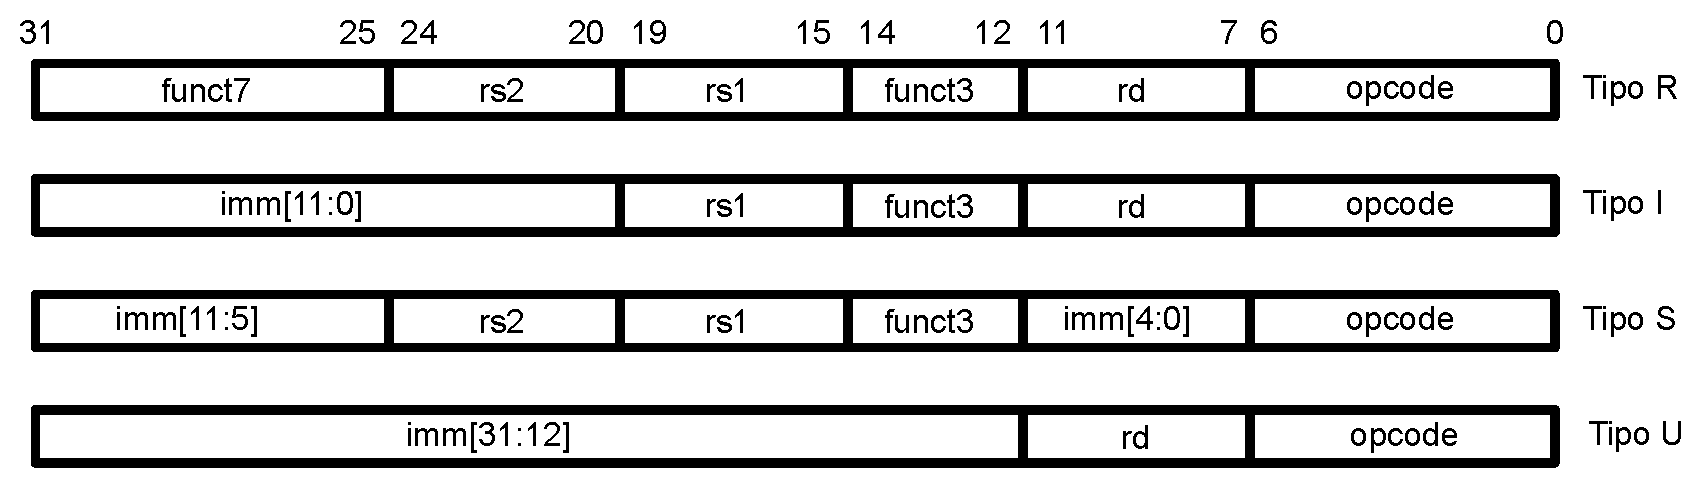
\includegraphics[scale=0.54]{figuras/instrucaoRISC-V.pdf}
     \fonte{Adaptado de \cite{riscv_manual_2026}}%% Fonte adaptada
\end{figure}

Para a execução da maioria das instruções de um processador, é indispensável a utilização da Unidade Lógica e Aritmética (ALU, do inglês \textit{Arithmetic Logic Unit}). A ALU é o componente central de processamento de dados do circuito, no qual são reunidos os blocos lógicos necessários para realizar operações aritméticas (como soma e subtração) e operações bit a bit (como deslocamentos e funções lógicas \textit{AND}, \textit{OR} e \textit{XOR}) \cite{hennessy2017organizacao}. 

Para realizar uma operação na ALU, é necessário fornecer três conjuntos de entradas: duas entradas de dados de $N$ bits de largura e uma entrada de controle de $x$ bits, responsável por determinar a operação. Após qualquer alteração em uma de suas entradas, a saída contendo $N$ bits é prontamente atualizada. A quantidade de bits de dados ($N$) que a ALU suporta é estabelecida pelas especificações da ISA, assim como o número de operações diferentes que o componente deve suportar. Consequentemente, a largura do sinal de controle ($x$) depende diretamente dessas operações obrigatórias mapeadas pela arquitetura, dado que cada valor binário representa uma operação específica \cite{hennessy2017organizacao}.

Antes que as instruções e os dados cheguem à ALU, é necessário que eles estejam armazenados em estruturas internas do próprio processador, garantindo que o acesso ocorra dentro de um único período de \textit{clock}. Para essa finalidade, são utilizadas as memórias de dados e de instruções. Essas duas memórias são fisicamente separadas para permitir que, em um mesmo ciclo de \textit{clock}, o processador realize a busca da instrução e, se necessário, efetue a leitura ou escrita na memória de dados. Essa simultaneidade de acesso é um requisito indispensável para o desenvolvimento deste trabalho, visto que o processador operará sob o modelo de ciclo único \cite{hennessy2017organizacao}.

Para realizar a comunicação entre o processador e os demais componentes do sistema, tornam-se necessários os dispositivos de Entrada e Saída (I/O, do inglês \textit{input} e \textit{output}). Atualmente, não é comum o uso de uma única central para todos os periféricos, mas sim de interfaces e controladores específicos para cada tipo de barramento \cite{silva2024arquitetura}. Como o projeto deste trabalho será implementado em uma placa FPGA, os dispositivos periféricos com os quais o processador se comunicará serão simplificados, consistindo dos próprios LEDs e chaves (\textit{switches}) integrados à placa de desenvolvimento.

Com a compreensão da evolução histórica dos computadores, o detalhamento das filosofias de ISAs e a definição dos blocos estruturais que compõem o modelo de ciclo único do RV32I, consolida-se a base teórica necessária para o desenvolvimento do hardware proposto. Diante desse cenário conceitual, torna-se igualmente importante analisar como a literatura recente tem abordado a implementação de processadores baseados na arquitetura RISC-V em matrizes de portas programáveis (FPGAs). Dessa forma, a próxima subseção apresenta uma revisão de trabalhos correlatos, estabelecendo um comparativo técnico que servirá de referência para as decisões de projeto adotadas neste trabalho.

\section{Trabalhos relacionados}
\label{sec:trabalhosRelacionados}

A literatura acadêmica apresenta diversas abordagens sobre a projeção, validação e aplicação prática de processadores baseados na arquitetura aberta RISC-V. Investigar o panorama recente permite compreender desde o teto de desempenho dessa tecnologia em sistemas complexos até as restrições físicas de frequência, área e consumo que envolvem o mapeamento de núcleos básicos em lógica programável.

No cenário atual, o ecossistema RISC-V tem se consolidado em setores de computação de alto desempenho e de aceleração de Inteligência Artificial. \citeonline{gorgonho2025uma} apresentaram uma revisão do estado da arte sobre o uso dessa ISA em ambientes de supercomputação e servidores de alta densidade. Os autores detalharam experimentos práticos como o \textit{cluster} italiano \textit{Monte Cimone V2}, o qual integra múltiplos computadores baseados em RISC-V para computação de alto desempenho (HPC, do inglês \textit{High-Performance Computing}); e arquiteturas comerciais como os aceleradores \textit{Tenstorrent Tensix}, que empregam arranjos de múltiplos núcleos para otimizar o fluxo de dados em cargas de trabalho de redes neurais, um modelo de inteligencia artificial (AI, do inglês \textit{Artificial Intelligence}). Esse panorama demonstra a escalabilidade e a maturidade global da arquitetura, justificando o interesse acadêmico e industrial na pesquisa detalhada de seus núcleos fundamentais.

Em contrapartida aos sistemas de altíssimo desempenho baseados em grandes agrupamentos de chips, a busca por eficiência e inovação também ocorre no escopo do projeto individual do processador. Nessa linha, \citeonline{mendes2025torvs} propuseram o TORVS, um núcleo baseado no conjunto básico RV32I que adota uma abordagem superescalar \textit{in-order} com vazão dupla (\textit{dual-issue}). Este modelo de processamento superescalar é uma variante do modelo de processamento em \textit{pipeline}, possuindo duas vias de execução paralelas que operam em ordem estrita, o que permite despachar e executar até duas instruções simultaneamente, diferenciando-se dos modelos tradicionais de via única. O projeto foi desenvolvido em linguagem SystemVerilog e validado fisicamente em uma matriz de portas programáveis (FPGA Intel DE10-Standard), com o objetivo principal de reduzir o indicador de Ciclos por Instrução (CPI, do inglês \textit{Cycles Per Instruction}).

Contudo, os autores observaram que a duplicação das vias de execução exige circuitos de controle e de desvio significativamente complexos. Na prática, essa complexidade microarquitetural gerou um gargalo no caminho de dados que limitou a frequência máxima de \textit{clock} do chip entre 70 e 90 MHz. Adicionalmente, por não integrar hardware específico para realizar multiplicações, o TORVS apresentou baixo desempenho em tarefas complexas, como a multiplicação de matrizes. Apesar das limitações em computação intensiva, o modelo provou-se altamente eficiente e superior aos processadores de via única convencionais ao executar instruções lógicas e fluxos de controle cotidianos mais simples.

Focado no cenário de ecossistemas de baixo consumo, o trabalho de \citeonline{Arul2024implementation} realizou a implementação completa de um processador funcional baseado no conjunto de instruções RV32I em ciclo único. Utilizando uma FPGA AMD Artix-7 para a prototipagem inicial, o circuito alcançou uma frequência máxima de operação de 32 MHz, apresentando um consumo de potência estimado em apenas 7,9 mW. Posteriormente, o projeto foi manufaturado em um chip com tecnologia CMOS de 65 nm, atingindo uma frequência máxima de 200 MHz; contudo, os autores ressaltam que o processo de \textit{tapeout} e o design físico de um ASIC são altamente trabalhosos, caros e complexos. Esse cenário valida a decisão metodológica deste trabalho, que adotará a plataforma Artix-7, limitando-se ao escopo da lógica programável por questões de viabilidade prática e de custo-benefício.

Complementando a análise de viabilidade em lógica programável, no trabalho \citeonline{depaula2025estudo}, os autores projetaram em Verilog HDL um processador RISC-V de ciclo único voltado para sistemas embarcados, utilizando a ferramenta Intel Quartus Prime para mapeamento e síntese na placa de desenvolvimento FPGA DE10-Lite. Por meio de simulações no \textit{software} ModelSim e validação em \textit{hardware} com rotinas em linguagem \textit{assembly}, o estudo detalhou os desafios práticos envolvidos na sincronização de sinais de controle. Semelhante ao esperado durante o desenvolvimento deste TCC, os autores reportaram falhas de temporização (\textit{timing}) durante a execução física, as quais foram mitigadas por meio de ajustes iterativos na lógica dos multiplexadores e nos caminhos críticos coordenados pela unidade de controle.

Expandindo as fronteiras para sistemas de validação de hardware, \citeonline{julio2024processorCI} propuseram o \textit{ProcessorCI}, uma infraestrutura automatizada que integra conceitos de integração contínua ao teste físico de processadores RISC-V em FPGAs de múltiplos fornecedores, como AMD Xilinx, Intel e Lattice. O ambiente utiliza o \textit{software} Jenkins para gerenciar um fluxo que automatiza a síntese do código de descrição de hardware, realiza o \textit{download} do arquivo de configuração para as placas físicas e injeta programas de teste gerados por ferramentas de estímulo aleatório. Módulos de hardware auxiliares foram projetados dentro da lógica programável para atuar como pontes de comunicação, controlando de forma não invasiva os sinais de \textit{clock}, \textit{reset} e os barramentos do núcleo processador. O trabalho demonstra o benefício de estabelecer rotinas rigorosas e automatizadas de teste direto no hardware, assegurando o correto funcionamento do circuito durante as etapas de escrita e modificação do código.

Esses trabalhos demonstram que, desde o alto desempenho em supercomputadores até a exploração de microarquiteturas embarcadas, a arquitetura RISC-V exige tanto uma compreensão clara de seu comportamento sistêmico quanto a aplicação de estratégias consistentes de teste em hardware. Tais referências estabelecem as diretrizes e os limites de projeto indispensáveis para avaliar a fidelidade física e o posicionamento técnico do processador RV32I desenvolvido neste documento.